\documentclass[11pt,british,a4paper]{report}
%\pdfobjcompresslevel=0
\usepackage{pythontex}
\usepackage[usenames,dvipsnames]{xcolor}
\usepackage[includeheadfoot,margin=0.8 in]{geometry}
\usepackage{siunitx,physics,cancel,upgreek,varioref,listings,booktabs,pdfpages,ifthen,polynom,todonotes}
%\usepackage{minted}
\usepackage[backend=biber]{biblatex}
\DefineBibliographyStrings{english}{%
      bibliography = {References},
}
\addbibresource{sources.bib}
\usepackage{mathtools,upgreek,bigints}
\usepackage{babel}
\usepackage{graphicx}
\graphicspath{{./}{./e/}}
\usepackage{float}
\usepackage{amsmath}
\usepackage{amssymb,epstopdf}
%\usepackage{fouriernc}
% \usepackage[T1]{fontenc}
% \usepackage{mathpazo}
% \usepackage{inconsolata}
%\usepackage{eulervm}
%\usepackage{cmbright}
\usepackage{fontspec}
\usepackage{unicode-math}
\setmainfont{Tex Gyre Pagella}
\setmathfont{Tex Gyre Pagella Math}
\usepackage{fancyhdr}
\usepackage[utf8]{inputenc}
\usepackage{textcomp}
\usepackage{lastpage}
\usepackage{microtype}
\usepackage[linktoc=all, bookmarks=true, pdfauthor={Anders Johansson},pdftitle={FYS4460 Project 2}]{hyperref}
\usepackage{tikz,pgfplots,pgfplotstable}
\usepgfplotslibrary{colorbrewer}
\usepgfplotslibrary{external}
\tikzexternalize[prefix=data/]
\pgfplotsset{cycle list/Set1}
\pgfplotsset{compat=1.8}
\renewcommand{\CancelColor}{\color{red}}
\let\oldexp=\exp
\renewcommand{\exp}[1]{\mathrm{e}^{#1}}
\renewcommand{\Re}[1]{\mathfrak{Re}\ifthenelse{\equal{#1}{}}{}{\left(#1\right)}}
\renewcommand{\Im}[1]{\mathfrak{Im}\ifthenelse{\equal{#1}{}}{}{\left(#1\right)}}
\renewcommand{\i}{\mathrm{i}}
\newcommand{\tittel}[1]{\title{#1 \vspace{-7ex}}\author{}\date{}\maketitle\thispagestyle{fancy}\pagestyle{fancy}\setcounter{page}{1}}

% \newcommand{\deloppg}[2][]{\subsection*{#2) #1}\addcontentsline{toc}{subsection}{#2)}\refstepcounter{subsection}\label{#2}}
% \newcommand{\oppg}[1]{\section*{Oppgave #1}\addcontentsline{toc}{section}{Oppgave #1}\refstepcounter{section}\label{oppg#1}}

\labelformat{section}{#1}
\labelformat{subsection}{exercise~#1}
\labelformat{subsubsection}{paragraph~#1}
\labelformat{equation}{equation~(#1)}
\labelformat{figure}{figure~#1}
\labelformat{table}{table~#1}

\renewcommand{\footrulewidth}{\headrulewidth}

%\setcounter{secnumdepth}{4}
\renewcommand{\thesection}{Oppgave \arabic{section}}
\renewcommand{\thesubsection}{\alph{subsection})}
\renewcommand{\thesubsubsection}{\arabic{section}\alph{subsection}\roman{subsubsection})}
\setlength{\parindent}{0cm}
\setlength{\parskip}{1em}

\definecolor{bluekeywords}{rgb}{0.13,0.13,1}
\definecolor{greencomments}{rgb}{0,0.5,0}
\definecolor{redstrings}{rgb}{0.9,0,0}
\lstset{rangeprefix=\#/,
    rangesuffix=/\#,
    includerangemarker=false}
\renewcommand{\lstlistingname}{Kodesnutt}
\lstset{showstringspaces=false,
    basicstyle=\footnotesize\ttfamily,
    keywordstyle=\color{bluekeywords},
    commentstyle=\color{greencomments},
    numberstyle=\color{bluekeywords},
    stringstyle=\color{redstrings},
    breaklines=true,
    texcl=true
}
\colorlet{DarkGrey}{white!20!black}
\newcommand{\eqtag}[1]{\refstepcounter{equation}\tag{\theequation}\label{#1}}
\hypersetup{hidelinks=True}

\sisetup{detect-all}
\sisetup{exponent-product = \cdot, output-product = \cdot,per-mode=symbol}
% \sisetup{output-decimal-marker={,}}
\sisetup{round-mode = off, round-precision=3}
\sisetup{number-unit-product = \ }

\allowdisplaybreaks[4]
\fancyhf{}

\rhead{Project 2}
\rfoot{Page~\thepage{} of~\pageref{LastPage}}
\lhead{FYS4460}

%\definecolor{gronn}{rgb}{0.29, 0.33, 0.13}
\definecolor{gronn}{rgb}{0, 0.5, 0}

\newcommand{\husk}[2]{\tikz[baseline,remember picture,inner sep=0pt,outer sep=0pt]{\node[anchor=base] (#1) {\(#2\)};}}
\newcommand{\artanh}[1]{\operatorname{artanh}{\qty(#1)}}
\newcommand{\matrise}[1]{\begin{pmatrix}#1\end{pmatrix}}


\pgfplotstableset{1000 sep={\,},
                      assign column name/.style={/pgfplots/table/column name={\multicolumn{1}{c}{#1}}},
                      every head row/.style={before row=\toprule,after row=\midrule},
                      every last row/.style={after row=\bottomrule},
                      columns/n/.style={column name={\(n^*\)},column type={r}},
                      columns/N/.style={column name={\(N\)},sci},
                      columns/logN/.style={column name={\(\log(N)\)}},
                      columns/logn/.style={column name={\(\log(n^*)\)}}
                      }

\newread\infile

%start
\begin{document}
\title{FYS4460: Project 1}
\author{Anders Johansson}
%\maketitle

\begin{titlepage}
%\includegraphics[width=\textwidth]{fysisk.pdf}
\vspace*{\fill}
\begin{center}
\textsf{
    \Huge \textbf{Project 2}\\\vspace{0.5cm}
    \Large \textbf{FYS4460 - Disordered systems and percolation}\\
    \vspace{8cm}
    Anders Johansson\\
    \today\\
}
\vspace{1.5cm}

\includegraphics{uio.pdf}\\
\vspace*{\fill}
\end{center}
\end{titlepage}
\null
\pagestyle{empty}
\newpage

\pagestyle{fancy}
\setcounter{page}{1}



%   __ _
%  / _` |
% | (_| |
%  \__,_|
%
\subsection{}
I reused the argon script from project 1, but changed the size of the system and the parameter of the lattice command. According to the project description, the lattice spacing should be \(a=\SI{5.72}{\angstrom} = \py{round(5.72/3.405,2)}\sigma\), giving a reduced density (the parameter of the \texttt{lattice} command) of
\[
    \rho^* = \rho\sigma^3 = \frac{4}{\qty(a/\sigma)^3} = \frac{4}{\py{round(5.72/3.405,2)}^3} = \py{round(4/(5.72/3.405)**3,2)}.
\]

\subsection{}
The system was first thermalised for a certain number of timesteps, determined by looking a the visualisations in the previous exercise. A cylinder was then created with the given dimensions, and the atoms inside were selected as a group. The remaining atoms were then given zero velocity for visualisation purposes and excluded from the integration. Visual inspection in Ovito shows that this approach works.

\subsection{}
I considered many options for making spheres with random positions and radii, and ended up using the \texttt{python} command in LAMMPs. This runs a Python function during the execution of the LAMMPs script. The funcion receives a pointer to a LAMMPs object, which it uses to extract variables and run commands.

The important part of the LAMMPs script is
\lstinputlisting[linerange={snippetstart-snippetend}]{cd/in.script}
The first \texttt{python} command defines the function \texttt{make\_spheres}, found in the \texttt{file make\_spheres.py}. This function takes \texttt{1} argument, \texttt{SELF}, which is a pointer (\texttt{p}) to the current LAMMPs object. The second \texttt{python} command runs the Python function. The \texttt{matrix} group is defined by the Python function as the atoms inside the spheres. The content of \texttt{make\_spheres.py} is the simple function
\lstinputlisting[language=Python]{cd/make_spheres.py}
Periodic boundary conditions are fully enforced by creating all relevant periodic images of each sphere. Unfortunately, the approach of using the \texttt{python} command inside LAMMPs to run LAMMPS commands does not work well with MPI, so the simulation is run serially.

Visualisation of the result was done by colour coding the atoms according to the magnitude of their velocities, where the lower bound is zero and the upper bound is a very small number. See \vref{fig:spheres}.
\begin{figure}[tbh]
    \centering
    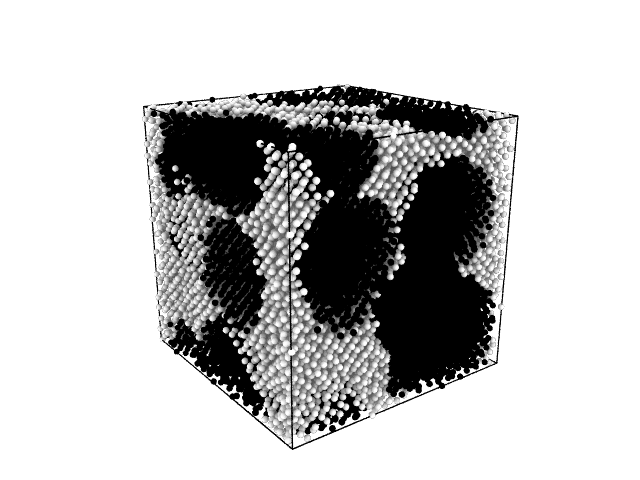
\includegraphics[width=0.5\textwidth]{cd/spheres.png}
    \caption{Visualisation of the randomly placed spheres.}%
    \label{fig:spheres}
\end{figure}

\subsection{}
See the above exercise.

\subsection{}
Armed with the \texttt{python} command discovered in the previous exercise, I used the LAMMPs commands
\lstinputlisting[linerange={snippetstart-snippetend}]{e/in.script}
The variable \texttt{is\_moving} is set to \(1\) for all atoms in the group \texttt{moving} and \(0\) for all atoms in the matrix. The Python function is
\lstinputlisting[language=Python]{e/delete_half_of_moving.py}
Halfway through writing this, I discovered that LAMMPs actually has built-in commands for deleting a certain fraction of the particles in a region, but at that point, there was no turning back. One difficulty of extracting values from \texttt{lammps} objects is the type of the values returned, which for arrays is a pointer to the underlying C++ structures. This must be converted using \texttt{numpy.ctypeslib.as\_array}.
\begin{pycode}
with open("e/data/beforedeletion.dat","r") as infile1, open("e/data/afterdeletion.dat","r") as infile2:
    before = infile1.read()
    after = infile2.read()
res = r"\(\num{%s}\) and \(\num{%s}\)" % (before, after)
\end{pycode}

The files written by the \texttt{print} commands in the LAMMPs snippet above contain \py{res}, showing that the number of atoms not in the matrix is indeed halved when the Python function is executed.








































\nocite{*}
\printbibliography{}
\addcontentsline{toc}{chapter}{\bibname}
\end{document}
